




\chapter{Conclusion}\label{conclusion}

\section{Future Work}\label{future-work}

\subsection{Dynamic target rejection}\label{dynamic-target-rejection}

\subsection{Online mapping}\label{online-mapping}

The proof of concept implementation processes pre-recorded data. However
the algorithm is by no means limited to offline processing. Being very
much iterative and range scan line based it requires only the knowledge
of current and past, but not future scans. A live version of the
algorithm was not built, because the implementation was done in Matlab,
which does not run on arm processors natively. Matlab's Robotics Toolbox
does include a way to receive ROS messages live, but it is very slow and
would miss a lot of messages. This was tested by replaying a rosbag,
which works only at less than 10\% replay speed. This means that a 6
minute recording takes around 60 minutes to process. On the other hand,
just reading in all the messages in a rosbag takes around 3 minutes,
which is the reason the implementation was not done live. In a real
system (i.e.~not replayed from a rosbag) sending raw scan messages over
the network requires a lot of bandwidth, so the sampling frequency also
drops considerably.

An online system would probably have to be designed as a ROS node that
runs on the embedded platform.

Another topic that needs to be looked at for an online version is the
size of the reprojection map. It should automatically expand if a wider
area is necessary. This could be handled in a nice way with ROS's
\texttt{nav\_msgs/OccupancyGrid} messages and/or the
\href{http://wiki.ros.org/grid_map}{grid\_map package}. This would also
allow pretty and useful visualizations with RViz.

\subsection{ROS nodelet}\label{ros-nodelet}

The \texttt{omniradar\_node} ROS node spends quite some time on copying
the radar echo into the ros message that is to be sent out. As Austin
Hendrix points out in
\href{https://answers.ros.org/question/208801/how-to-have-no-copy-publishing-over-multiple-cores/?answer=208805\#post-id-208805}{ROS
answers}, ``ROS doesn't provide intra-process, zero-copy publishing.
Nodelets can be run multi-threaded, so it is possible to have zero-copy
between different nodelets within a single nodelet manager''. Recording
a rosbag still involves copying the data, but in an online system a
nodelet-based reprojecting algorithm can be expected to bring a
reasonable performance improvement.

\subsection{Auto-thresholding}\label{auto-thresholding}

\subsection{Realtime}\label{realtime}

An obstacle sensor's job is to provide information on impeding
collisions before it's too late. Thus it would be great to have the
system run under realtime constraints, so it can guarantee range
scanning and reprojection mapping to be finished within a known time
frame.

\subsection{Dynamic changing of sweep time and
bandwidth}\label{dynamic-changing-of-sweep-time-and-bandwidth}

\subsection{Interference
Investigation}\label{interference-investigation}

Since the 60 GHz band is ISM, other sources can be present, e.g.~the
IEEE 802.11ad standard \cite{IEEE2014} (``WiGig'') which enables very
high throughput wireless LAN operation in frequencies around 60GHz.
Commercial products using WiGig are already available and could cause
some interference with the 60GHz radar sensor. Detecting or avoiding
interference in the range signal would be an important topic if this
causes a lot of trouble.

\subsection{Ultrasound}\label{ultrasound}

Usually, ultrasound sensors measure the distance to the closest object.
However, K.C. Lee's project log of their ``Sonar for the visually
impaired'' project \cite{Lee2015} shows how cheap sensors can be hacked
to read a range profile that looks very similar (see figure \#REF) to
what is used for the radar reprojection method. It might be possible to
adapt the algorithms in this thesis to use ultrasound sensors.
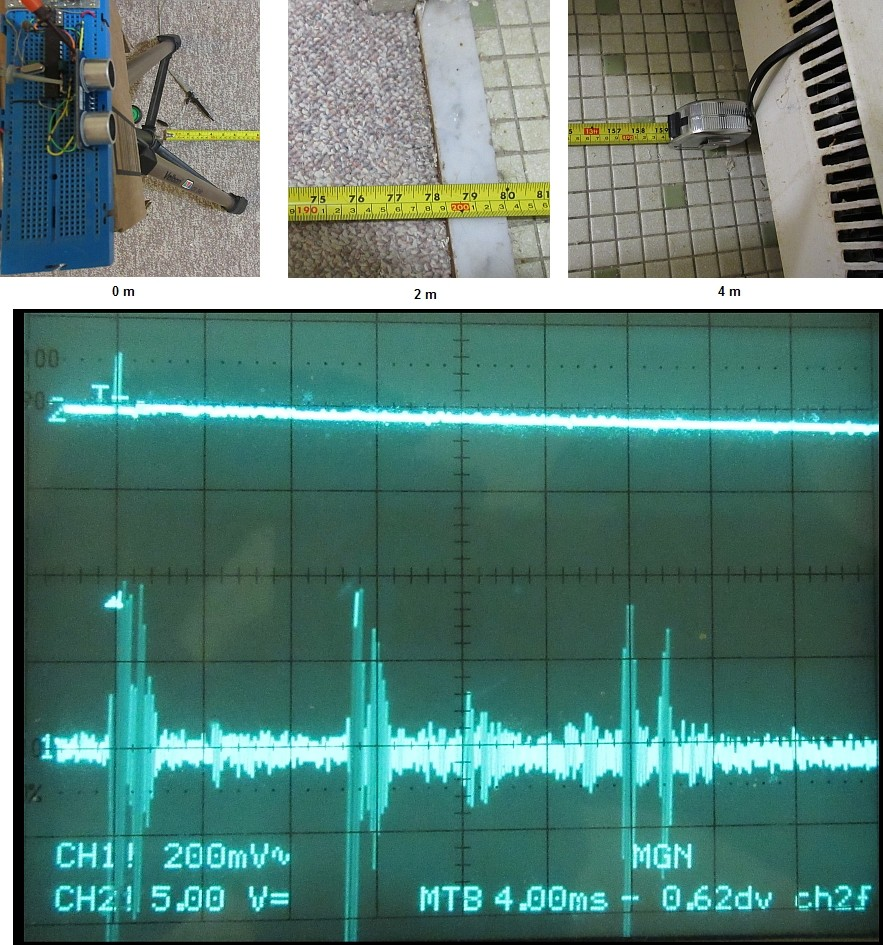
\includegraphics[width=0.5\textwidth]{pictures/had_us}

Most ultrasound range sensors use the time of flight of a pulsed echo,
but FMCW-based ultrasound modules have been proposed
\cite{Battaglini2014} recently. With a range resolution of
\[dR = \frac{c_{sound, air}}{2 BW} = \frac{330 \frac{m}{s}}{2\cdot 12.5kHz} = 1.32 cm\]
the proposed sensor would be comparable to the Omniradar sensor's range
resolution and accuracy. However, for measurements to be very accurate
the speed of sound in air must be known as it depends on humidity and
temperature \cite{Bohn1987}.

For forward-facing geometry DOA is necessary to resolve the sign of the
reprojection angle. Sound waves do not not carry phase information, but
with a transducer array, direction of arrival can still be estimated
\cite{Kunin2010}.

Extension to ultrasound sensors would be a very interesting topic for
further work.

It might even be possible to use light waves with interferometric
modulated flash lidars and the right optics.

\subsection{3D case}\label{d-case}

Chapter \#REF describes the general geometry for 2D-cases. However, it
is possible to extend the concept to the three dimensional space if a
radar has more than two non-collinear receiving antennas, like
visualized in figure \#REF. Horizontal DOA would be measured between
antennas at positions \(Rx1\) and \(Rx2\) while vertical DOA would be
measured between \(Rx1\) and \(Rx3\).
%\includesvg[width=0.5\textwidth]{"diagrams/2D-DOA"}
Reprojection mapping could then be used to build 3D occupancy maps. The
reprojection angle \(\alpha\) would then describe a circle at distance
\(R~cos(\alpha)\) around the radar path, on which the detected target
lies. Direction of arrival in horizontal and vertical planes would then
have to be used to pinpoint the target location on the circle.
%\includesvg[width=0.5\textwidth]{"diagrams/3Dcase"}
This holds also for the 2D-case: The possible locations for targets are
then at the intersection of reprojection cone circle and floor plane.

This would be useful on vehicles moving in 3D space, like the TUM RCS's
\href{https://www.rcs.ei.tum.de/forschung/mart/}{Modular Airborne
Real-Time Testbed (MART)} that was also used in other research and
publications \cite{Becker2015}.

\subsection{Single receive antennas on multiple
sensors}\label{single-receive-antennas-on-multiple-sensors}

Direction of arrival is a good solution to resolve the ambiguities
presented in the general 2D-case \#REF and 3D-case \#REF geometry for a
sensor with a sufficient number of antennas. However, it should also be
possible to use multiple, spatially separated sensors instead. Each
sensor measures a reprojection angle. A target visible to both sensors
can then be localized unambiguously with triangulation.



3D scenario. standard case: two intersecting spheres --\textgreater{}
intersection circle doppler reprojection case: angle --\textgreater{}
cones with intersecting base edge -\textgreater{} two interesection
points (DOA to resolve, or high flying drone to assume)

\section{Conclusion}\label{conclusion-1}

Mobile robots still struggle to detect some obstacles that are invisible
to their conventional sensors. Radar sensors have a big potential to
improve obstacle avoidance. With reprojection mapping, this thesis
proposes a novel method to create an obstacle map without having to
steer the radar beam.

A proof-of-concept implementation of the reprojection mapping produced
obstacle maps from the radar scans of the experiments for this thesis.
The maps prove that some previously undetectable obstacles, like glass
walls and office chair legs, can now be detected and mapped.

The next step on the way to a mobile indoor robot proficiently
navigating real-world environments should be the implementation of an
online version of reprojection mapping. This will also show if the
results need to be further improved with more advanced noise rejection.

\ldots{}